% ---------------------------------------          Preamble
\documentclass[
	fontsize=12pt,
	paper=a4,
	twoside=false,
	numbers=noenddot,
	plainheadsepline,
	toc=listof,
	toc=bibliography
]{scrartcl}

\usepackage[english]{babel} 

\usepackage{amssymb}
\usepackage{amsmath}
\usepackage{array}

\usepackage{placeins}
\usepackage{float}

\usepackage{graphicx}
\restylefloat{figure}
\usepackage{caption}
\usepackage{subcaption}
%\usepackage{subfigure} 
\usepackage{tikz}

%\usepackage{pdfpages} % insert images saved as pdf

% pseudo algorithms
\usepackage[ruled,vlined]{algorithm2e}

% lscape.sty Produce landscape pages in a (mainly) portrait document.
\usepackage{lscape}

\usepackage{hyperref}

\setlength{\parindent}{0pt}

\usepackage[sort, numbers]{natbib}
% ---------------------------------------          New commands
%\newcommand{\argmin}{\operatornamewithlimits{argmin}}
\def\argmax{\mathop{\rm argmax}}						% argmax
\def\argmax{\mathop{\rm argmin}}						% argmin
\def\median{\mathop{\rm median}} 						% median
\def\dist{\mathop{\rm dist}} 						    % dist


\usepackage{array}
\newcolumntype{L}[1]{>{\raggedright\let\newline\\\arraybackslash\hspace{0pt}}m{#1}}
\newcolumntype{C}[1]{>{\centering\let\newline\\\arraybackslash\hspace{0pt}}m{#1}}
\newcolumntype{R}[1]{>{\raggedleft\let\newline\\\arraybackslash\hspace{0pt}}m{#1}}


\usepackage{xcolor} 
\newcommand\ToDo[1]{\textcolor{red}{#1}} 

% ------------------------------------------------------------------------------------------------------------
% ------------------------------------------------------------------------------------------------------------
% ------------------------------------------------------------------------------------------------------------

\begin{document}

\pagestyle{plain}
\pagenumbering{arabic}

% ------------------------------------------------------------------------------------------------------------
% ---------------------------------------          Title
\title{Graph Matching Framework}
\author{Ekaterina Tikhoncheva}
\date{} 

\maketitle 



% ------------------------------------------------------------------------------------------------------------
% ---------------------------------------        Experimantal Evaluation
\section{Experimental Evaluation}

\begin{figure}[ht] 
	\begin{subfigure}[b]{0.5\textwidth}
		\centering
		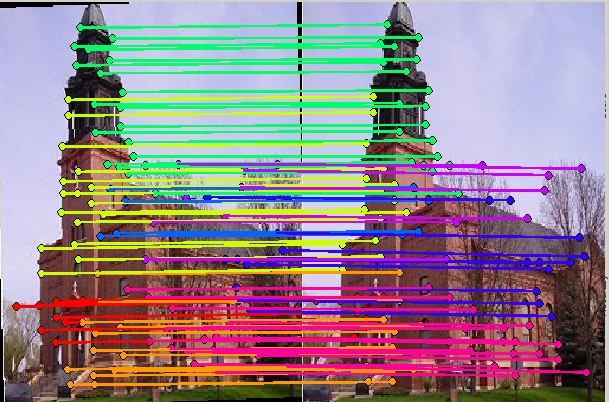
\includegraphics[scale=0.35]{fig/method1/test1/LL_it6.jpg} 
		\caption{$SM$ Previous version} 
	\end{subfigure}%% 
	\begin{subfigure}[b]{0.5\textwidth}
		\centering
		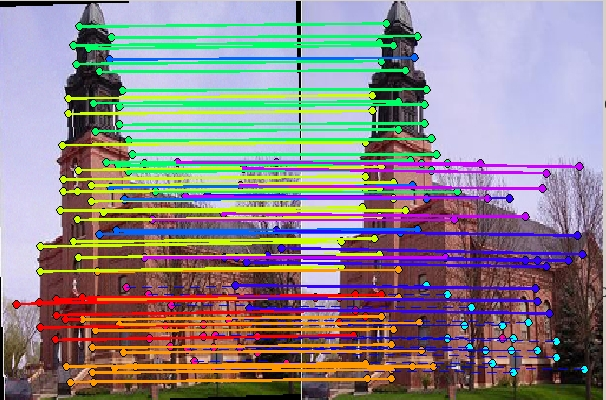
\includegraphics[scale=0.35]{test1/it6.jpg} 
		\caption{$SM$ New version} 
	\end{subfigure} 
	\caption{Result of the two-level graph matching approach after $6$ iterations }
\end{figure}

\begin{figure}[ht] 
	\begin{subfigure}[b]{0.5\textwidth}
		\centering
		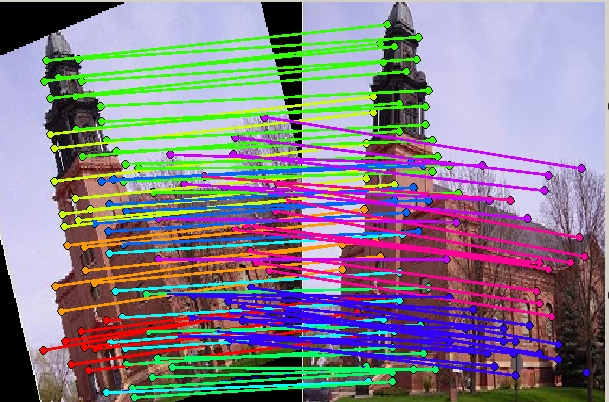
\includegraphics[scale=0.35]{fig/method1/test2/LL_it11.jpg} 
		\caption{$SM$ Previous version} 
	\end{subfigure}%% 
	\begin{subfigure}[b]{0.5\textwidth}
		\centering
		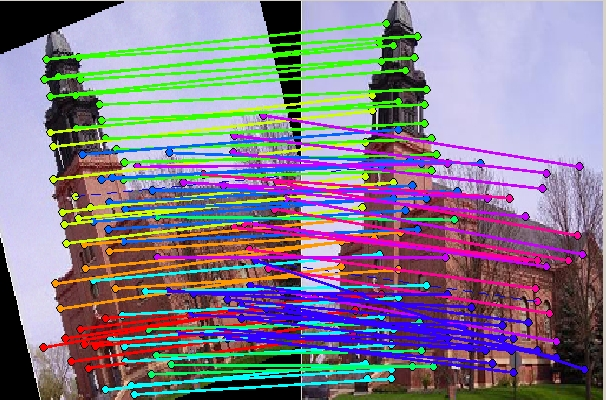
\includegraphics[scale=0.35]{test2/it11.jpg} 
		\caption{$SM$ New version} 
	\end{subfigure} 
	\caption{Result of the two-level graph matching approach after $11$ iterations }	
\end{figure}

\begin{figure}[ht] 
	\begin{subfigure}[b]{0.5\textwidth}
		\centering
		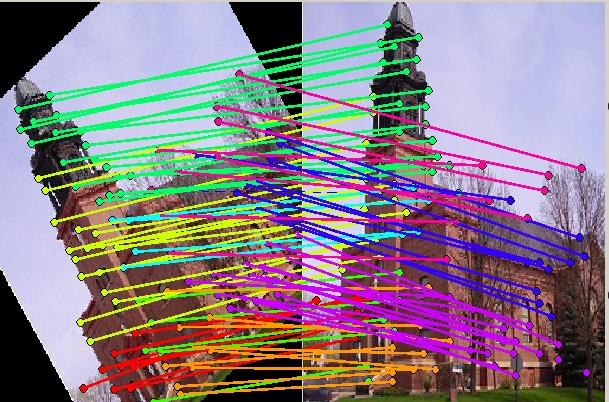
\includegraphics[scale=0.35]{fig/method1/test3/LL_it13.jpg} 
		\caption{$SM$ Previous version} 
	\end{subfigure}%% 
	\begin{subfigure}[b]{0.5\textwidth}
		\centering
		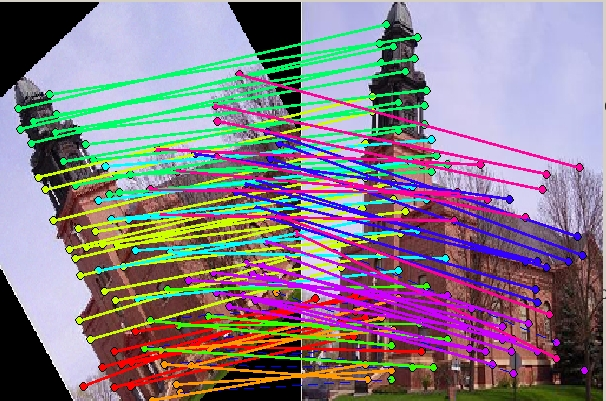
\includegraphics[scale=0.35]{test3/it11.jpg} 
		\caption{$SM$ New version} 
	\end{subfigure} 
	\caption{Result of the two-level graph matching approach after $13$ iterations }
\end{figure}

\newpage
	
\begin{table}
	[ht] \caption{Results of two-level Graph Matching Approach } \label{tab:stimuli}
	\begin{tabular}
		{|L{6cm}|L{6cm}|} \hline
%		              & \multicolumn{2}{c|}Higher Level} & \multicolumn{2}{c|}{Lower Level} \\ 
		Lower Level Convergence (previous version) &  Lower Level Convergence (new version)\\ \hline
		% first row
		\rule{0pt}{5cm}
		\parbox[b]{1em}{
			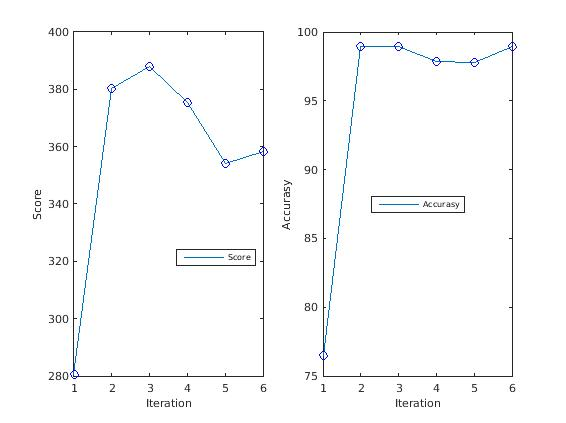
\includegraphics[scale = 0.28]{fig/method2/test1/accuracy_LL.jpg}} &
		\parbox[b]{1em}{
			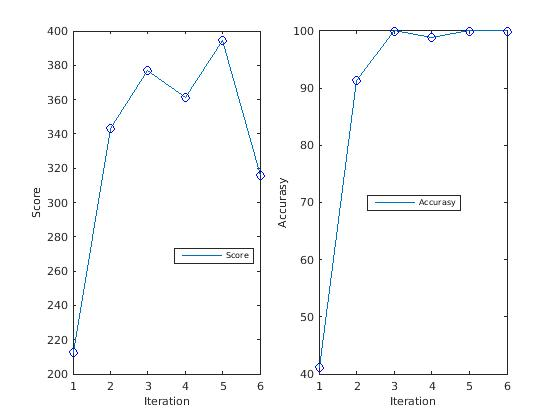
\includegraphics[scale = 0.28]{test1/accuracy_LL.jpg}} \\			
		\hline	
		
		\hline

		% second row
		\rule{0pt}{5cm}
    	\parbox[b]{1em}{
			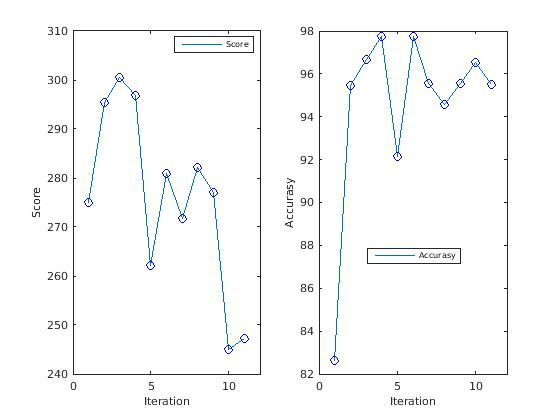
\includegraphics[scale = 0.28]{fig/method2/test2/accuracy_LL.jpg}} &
		\parbox[b]{1em}{
			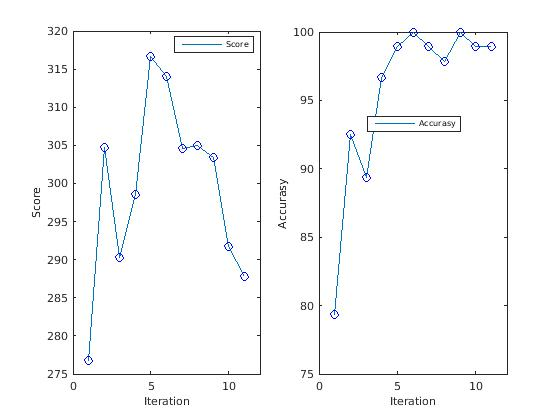
\includegraphics[scale = 0.28]{test2/accuracy_LL.jpg}}  \\
		\hline	

		% third row
		\rule{0pt}{5cm}
 		\parbox[b]{1em}{
			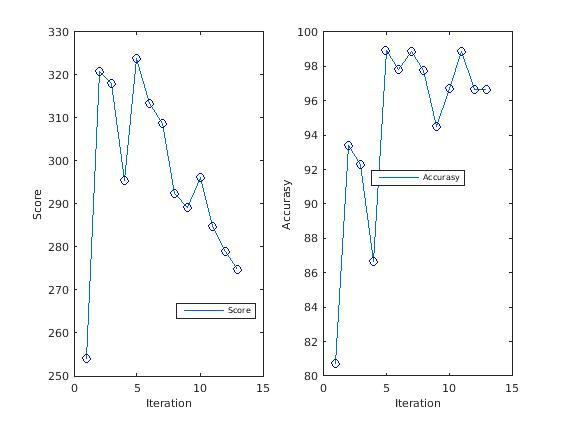
\includegraphics[scale = 0.28]{fig/method2/test3/accuracy_LL.jpg}} &
		\parbox[b]{1em}{
			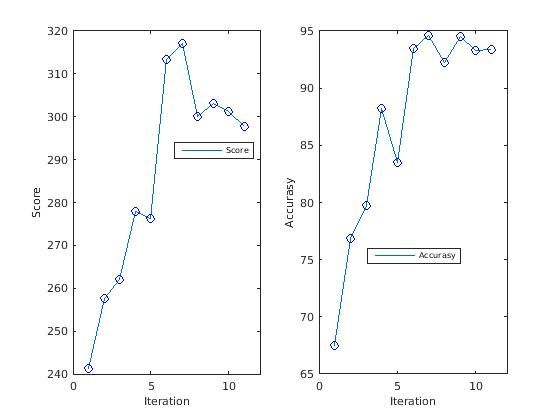
\includegraphics[scale = 0.28]{test3/accuracy_LL.jpg}}  \\
		\hline			
		
	\end{tabular}
\end{table}



% ------------------------------------------------------------------------------------------------------------
% ---------------------------------------        Bibliography
\bibliographystyle{abbrv}
\bibliography{bibliography}
	
\end{document}